

\subsection{Generelles}
- Titel und allgemein: 
In der Literatur gibt es die Begriffe  'time-of-flight' und 'transient current technqiue' fuer die selbe Methodik. 
Da die physikalische Messgroe3e ein Strom ist, und die Driftzeit eine aus dieser Messung abgeleitete Groe3e, finde ich den Begriff Transient current technique passender. Welchen Begriff bevorzugen Sie?

- In Kapitel 3 nehme ich Anpassungen vor, um die Transitzeit und die charakteristische Zeitkonstante zu bestimmen. 
Die Begruendung fuer die gewaehlten Funktionen kommen aber eigtl erst in Kapitel 4. 
Ist es Ihrer Meinung nach genug, jeweils auf Kapitel 4 zu verweisen? 
Eine andere Moeglichkeit waere es, im Kapitel 3 nur auf die Datenpunkte zu verweisen, und die Fit-Funtionen erst in Kapitel 4) zu erwaehnen. 

\subsection{Part I}


A1\\
Titel: Ich habe ``temperature- and electric field-dependent'' weggelassen, um den Titel weniger sperrig zu machen. 
Das kann natuerlich ganz leicht auch wieder geaendert werden. 

A2\\
Der Leser kennt zu diesem Zeitpunkt das Modell nicht, und somit auch nicht die Zeitkonsten. 
Eine Auflistung und Diskussion der Werte scheint hier also nicht sinnvoll. 
Dies kann erst in Part II geschehen. 
Der Absatz, der mit [] markiert ist, koennte also nach hinten wandern. 


\subsection{Part II}

B1\\
Neu formuliert.

B2\\
Ich schlage vor den Halbsatz ``depending weakly on the electric field'' zu streichen. Warum ist es noetig hier eine schwache Abhaengigkeit zu attestieren?

Noch wichtiger aber: Wie soll im exp.\ Teil gezeigt werden, dass die Bindungsenergie ca 80 meV betraegt, wenn der Fit, der dazu notwenig ist, erst durch das Modell motiviert wird?
Kann nicht mit einem generischen Bindungszustand diskutiert werden, der eine Aktivierungsenergie hat, die durch den Fit messbar wird? 

B3\\
Wieso ist es wichtig, dass hier nur FE in Frage kommen? Noch einmal, kann nicht mit einem generischen Bindungszustand diskutiert werden, der eine Aktivierungsenergie hat, die durch den Fit messbar wird? 
Das sollte m.M.n.\ fuer die dann folgende Formulierung ausreichend sein. 

B4\\
Die Sample sind nicht wirklich gelblich, siehe Dissertation Fig 4.1. Der Hersteller bescheinigt eine Verunreiigung von $<$ 1e14 1/cm3. Wuerde das nicht als Erklerung reichen?

B5\\
Ich habe es schon oefters erwaehnt, aber der induzierte Strom ist nicht einfach die driftende Stromdichte, siehe auch Shokley-Ramo-Theorem (z.B. meine Dissertation 3.2.1). 
Es fehlt das weighting potential $1/d$. 
Wenn eine Probeladung von genau $\e$ von einer Seite zur anderen driftet, ist die insgesamt induzierte Ladung genau $\e$ (Ladungserhaltung). 
Ihre Formel fuer N = 1 wuerde aber viel groe3ere Ladungen bedeuten, wenn der Detektor sehr dick waere und somit die Driftzeiten lang. 
Mit dem Faktor $1/d$ ist die induzierte Gesamtladung immer genau $\e$ (oder $N*\e$), unabhaengig von der Dicke, wie es sein sollte. 
Es muss im Paper dann auch irgendwann erwaehnt werden, dass von der Dichte $n$ zur Anzahl $N$ uebergegangen wird, durch raeumliche Integration,
 so dass der induzierte Strom auch wirklich ein Strom ist, und keine Stromdichte.
Ich schlage vor das Gro3buchstaben eine Anzahl beschreiben, und kleine Buchstaben Dichten.

Richtig muesste es also m.M.n.\ hei3en:

The electron concentration in the outer range at the end of the relaxation phase is called $\no(0)$, with a corresponding number $\No(0)$.
The resulting current measured at the anode is

\begin{equation}
 i(t) = q\No(0)v(t)/d. 
\end{equation}

\noindent
The electron package reaches the anode at the transit time $t'$, from then the current decreases linearly to zero in a time interval of  $\Delta t = \dpen/v$  since the incoming carriers flow into the anode.   

B6\\
Sie diskutieren spaeter, dass $\taub$ klein sei (1 ps), da $n_1$ gro3 ist, lassen dann aber den Term $1/\taub$ weg, obwohl doch mathematisch gesehen nach Ihrer Argumentation $1/\taudrift$ weggelassen werden koennte!
Dies muss unbedingt geklaert werden. 

B7\\
Nun sagen Sie, dass $n_1(0)$ klein sei gegen $n_0(0)$, um den Term $n_1 / \taub$ wegzulassen, und zwar ``directly after exciton formation''.
Zu diesem Zeitpunkt kann aber $\taub$ nicht mehr klein sein, da ja nun $n_1$ klein ist. 
Es werden also $\taub$ und $n_1$ vor und nach Thermalisierung herangezogen, um den Term generell wegzulassen. 
Das halte ich fuer problematisch, kann man den Term doch nur weglassen, wenn er zu allen Zeitpunkten kleiner waere. 
Da $\taub$ und $n_1$ aber invers proportional gekoppelt sind, gestaltet sich dies schwierig. 

Au3erdem: Wenn $n_1(0)$ klein ist (ca 1e15) und $\taub$ im ps Bereich, ist das Verhaeltnis $n_1 / \taub = $ 1e15 / ps aehnlich zu $n_0 / \tauzero = $ 1e18 / ns. 

B8\\
Siehe dazu mein Modell in Section7.
Vorallem: $\tauevap$ ist m.M.n.\ eher $\tauevap = \frac{1}{\sigma v n_V}\exppEx$, und nicht $\tauevap = \frac{1}{\sigma v n_1}\exppEx$.
Diese Abschaetzung fuehrt also nicht zu einem realistischen Wert fuer $\taub$, da $\taub$ in der Formel dann gar nicht mehr auftaucht. 
Siehe dazu auch die folgende Literatur: 
``Discharge of trapped electrons from MOS structures'', K. Yamabe and Y. Miura, Journal of Applied Physics 51, 6258 (1980), http://dx.doi.org/10.1063/1.327612, im Appendix, Formeln A1. 

B9\\
Wie erwaehnt, haben Sie diskutiert, dass $\taub$ klein ist, vernachlaessigen aber $1/\taub$ anstatt $1/\taudrift$. 

B10\\
Es fehlt wieder $1/d$, und es waere dann nicht der Strom, sondern eine Stromdichte, die den inneren Bereich verlaesst. 

B11\\
Siehe B10

B12\\
Das ist ``total inner'' charge. Ich aendere $Q$ in $\Qin$. 

B13\\
$\Nin$ muss ANZAHL sein. Die Einheit ist dann aber immernoch C*m, es fehlt wieder der Faktor 1/d. 
Die Dicke $d$ kuerzt sich also einfach raus, und es ist egal wie dick der Diamant ist. Die Dicke beinfluesst nur die Staerke des elektrischen Feldes, aber nicht die Gesamtladung. 

B14\\
Das Unterkapitel wurde von mir hinzugefuegt, um eine Vergleichbarkeit zu den Fit-Funktionen herzustellen. 

B15\\
Die Fit-Funktionen lauteten eigentlich $\propto \frac{\tauzero}{\taurec} = \frac{1}{1+\tauevap/\taurec}$. 
Es muesste also mindestens noch die Vereinfachung $\tauzero - \taudrift \approx \tauzero$ gemacht werden, damit wieder der Faktor wieder $\frac{\tauzero}{\tauevap}$ lautet. 
Intuitiver, und fuer den Leser verstaendlicher, sind die Integrale inklusive des Tails. 

B16\\
Wenn man erst einmal 80 meV annimmt, muss es an dieser Stelle revidiert werden. 
Aber welchen Vorteil hat das? 
Ich schlage vor, wir nennen erst einmal nur den Wert von 90 meV bei 500 V, 
 und interpretieren diesen erst in diesem Kapitel. 
Vorher kann geneisch von ``einer Aktivierungsenergie'' gesprochen werden. 

B17\\
Oder einfach:
We conclude that for the entire temperature range relevant to the discussion, i.e.\ $T<\SI{150}{\kelvin}$, one unique activation energy $\Ea$ does apply to the e-h plasma in our TCT experiment. 
(Ich wuerde es nicht ``electron charge collection measurement'' nennen, da es vorher entweder TCT oder ToF genannt wird.)

B18\\
``... in a pulse'', besser: ``in the initial ionisation volume'', der ``pulse'' beschreibt ja den Strom und nicht das Ionisationsvolumen. 

B18'\\
Die Wurzeln sind m.M.n.\ in Ihrem Manuskript falsch gesetzt. Ich habe nachgerechnet und komme auf folgende Ausdruecke:
\begin{equation}
 x_{\textrm{max}} = \sqrt{\frac{\e}{4\pi\varepsilon\varepsilon_0 \xi}}
\end{equation}

\noindent
und

\begin{equation}
 \Delta E(x_{\textrm{max}}) = -2\e^2 \sqrt{\frac{\xi}{4\pi\varepsilon\varepsilon_0 \e}}
\end{equation}


B19\\
Sollte das hier dann nicht ``FE bound within an EHD'' hei3en?

B20\\
Die Proben sind klar (siehe auch Foto in meiner Dissertation). 
Stickstofflevel werden vom Hersteller im 1 ppb Bereiceh angegeben, auch wenn diese nicht unabhaengig verifiziert wurden.

B21\\
Ausgehend von $ \frac{\nt}{\nl} = \frac{4}{2}\exp{(-\delta/\kB T)}$ komme ich nach mehrfachem Nachrechnen auf:

\begin{equation}
 n_t = \frac{N}{1+1/2 \exp{(+\delta/\kB T)}}, \qquad n_l = \frac{N}{1+ 2\exp{(-\delta/\kB T)}}
\end{equation}

\noindent
Bitte ueberpruefen Sie Ihre Berechnung. Z.B.\ haben Sie bei beiden Exponenten ein ``-'', was m.M.n.\ falsch ist. 

B22\\
Der Strom lautet dann

\begin{equation}
 j = j_{\textrm{t}} + j_{\textrm{l}} = \q\left( \nt \vt + \nl \vl \right) = \q N \xi \left( \frac{\mut}{1+1/2\exp{(+\delta/\kB T)}}  + \frac{\mul}{1+2\exp{(-\delta/\kB T)}}\right) 
\end{equation}

B23\\
``After some reformulation ....: ''\\
Nur mittels Umformung kann dies m.E.\ nicht passiert sein, oder ich verstehe es nicht. 
Der Strom $j$ kommt nun nicht mehr vor, und der Strom selbst sagt auch nichts ueber die Driftzeit, die ja von der Dicke der Probe abhaengt, aus.
 
Es wird wahrscheinlich eine weitere Bedingung benutzt: z.B. $\mu_{eff} = \frac{n_l \mul + n_t \mut}{N}$, und dann
\begin{equation}
 \ttr = \frac{d}{\mu_{eff}\xi} = \frac{d}{\xi \frac{n_l \mul + n_t \mut}{N}} = ...
\end{equation}

\noindent
Dann komme ich auch auf Ihre Formel. 
Ich wuerde aber nicht $\mu_1$ und $\mu_2$ verwenden, sondern $\mu_l$ und $\mu_t$.

B23'\\
Kann hier fuer $\mul$ die empirische Formel $\mu(E) = \frac{\mu_0 \xi}{1+ \frac{\mu_0 \xi}{\vsat}}$ benutzt werden?
Damit waere die feldabhaengige Streuung an optischen Phonon beschrieben. 
Die Niederfeldmobilitaet kann dann noch, siehe meine JAP Publikation, dargestellt werden als $\mu_0 (T) = (\frac{1}{\muaps} + \frac{1}{\munis})^{-1}$. 
Dann waeren die temperaturabhaengig Streuung an akustischen Phonon und die temperaturunabhaengig Streuung and neutralen Impurities beschrieben. 

B24\\
Ich hatte es so verstanden, dass die transversalen Valleys hoehere kinetische Energie haben. 
Bei Ihrer Formal komme ich auf
\begin{equation}
 \delta = \Delta E_{\textrm{kin}} = 1/2 \cdot\ml \vl^2 - 1/2 \cdot\mt \vt^2 = - 2\ml \vl^2
\end{equation}

\noindent
Ich wuerde vorschlagen, das $\delta$ anders herum zu definieren:
\begin{equation}
 \delta = \Delta E_{\textrm{kin}} = 1/2 \cdot\mt \vt^2 - 1/2 \cdot\ml \vl^2  = + 2\ml \vl^2
\end{equation}

\noindent
wie es auch in Ihrer Formel (14) steht. 

B25\\
Ich kann die Werte in der Tabelle nicht nachvollziehen.
Meine JAP-Publikation zeigt deutlich abweichende Werte von Ihrer Tabellem. 
Zur Klaerung habe ich den Plot oben (Fig.\ 17 ) hinzugefuegt. 
Es fehlt auch die Angabe, bei welcher Temperatur die Werte genommen wurden. 
Diese muessten dann im Fit auch temperaturabhaengig gemacht werden, also anstatt eines Vektors $\delta(\xi)$) eine Matrix $\delta(\xi,T)$. 
Was meinen Sie dazu?

\begin{figure}[tb]
 \centering
 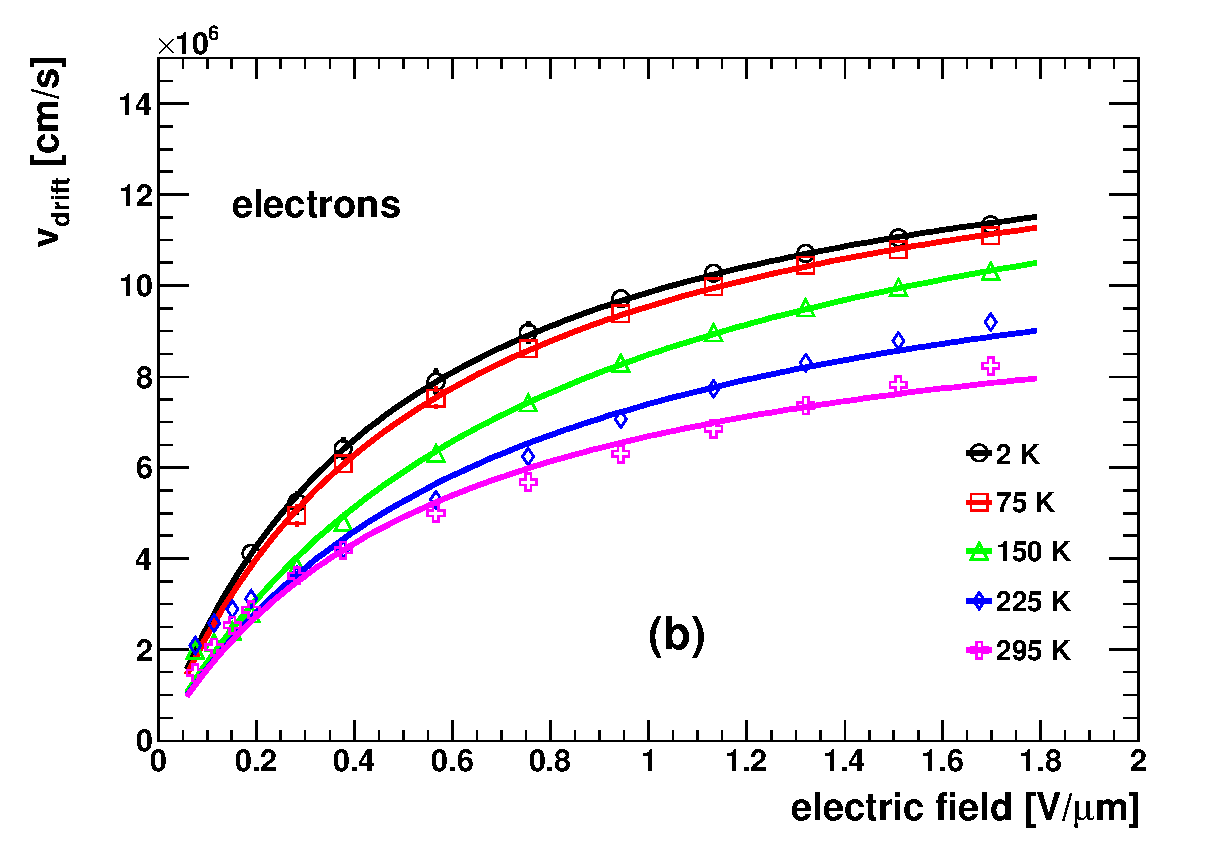
\includegraphics[trim=0 0 0 0, width=0.8\textwidth]{figures/MOBfitelecs.eps}
 \caption{}
\end{figure} 



B26\\
In der Tabelle wird nun das gemessene $\vdrift$ in Eq.\ (41) eingesetzt, um $\delta$ zu berechnen. 
In der Formal steht aber $\vl$, und nicht $\vdrift \equiv v_{eff}$.
Das vernachlaessigt vor allem die Mischung!
Waere es nicht besser, $v_{eff} = \mu_{eff}E$ anzunehmen, wieder mit $\mu_{eff} = \frac{n_l \mul + n_t \mut}{N}$,
 dann hat man in Kombination mit Eq.\ (41) ein Gleichungssystem mit 2 Gleichungen und 2 Unbekannten ($\delta$ und $\vl$, da $v_{eff}$ ja bekannt aus der Messung).
Mit $\delta' = \delta / \kB T$ erhalte ich
\begin{align}
 \delta' &= 2 m \vl^2 / (\kB T) \\
 v_{eff} &= \vl \cdot \left( \frac{1}{1+ 2\exp(-\delta')} + \frac{R}{1 + 0.5 \exp(+\delta')}\right)
\end{align}

\noindent
Diese System koennte man dann fuer verschiedene Feldstaerken und Temperaturen loesen und und jeweils $\delta(T;\xi)$ zu berechnen. 
Dies habe ich exemplarisch fuer T = 150\,K gemacht und der Tabelle hinzugefuegt. 
N.B.: Das Gleichungssystem habe ich jeweils numerisch geloest, um die Tabellenwerte zu erhalten. 

B27\\
Es wird mir (und deswegen vielleicht auch dem allgemeinen Leser) nicht klar, wie $\ttr$ in der Form Eq.\ (42) mit $t_{basic}$ zusammenhaengt, und welche Funktion nun ``these model curves'' sind. 
Eq.\ (43) enthaelt den Repopulation-Effekt nicht, und Eq.\ (42) nicht die Phononstreuung als Funktion der Temperatur. 
Au3erdem gibt es keinen formulierten, funktionalen Zusammenhang $\delta = \delta(T)$, damit eine stetige Kurve gezeichnet werden koennte. 
Dieser Zusammenhang koennte aus einem Fit an die Tabellenwerte von $\delta(T)$ entnommen werden, sogar fuer verschiedene Feldstaerken. 
Die Werte selbst liegen in Fig.\ 11 vor. 

B28\\
Ich habe den Teil $\left( 0.5 + \frac{0.6}{300\,T} \right)$ als Exponent dargestellt, ich hoffe dass dies richtig war. Bitte korrigieren Sie mich sonst. 

B28'\\
Ich bin der Meinung, dass die von Ihnen aufgezeigte Erklaerung nicht passt. 
Nimmt man $\taurec = $ 14\,ns an, und nimmt die Werte von $\taudrift$ im Bereich von ca 50\,ps..1\,ns, wird der Nenner $\taurec + \taudrift$ nicht gro3 genug, um das Verhaeltnis der gemessenen Ladung
 zur angenommenen Gesamtladung stark zu aendern.
Dafuer ist $\taurec$ zu gro3. 
Ich habe versucht diese Idee zu ``retten'', in dem ich angenommen habe, dass $\taurec \approx 1 / \sigma n_{\textrm{trap}} \vth$ mit $\vth \propto \sqrt{T}$. 
Dann waere $\taurec(\SI{300}{\kelvin}) = \SI{8}{\ns}$, aber auch das reicht noch nicht aus. 

B29\\
Meine Mobilitaetswerte (JAP) oder andere, z.B. Gaybrisch?


\subsection{Deswegen ...}
Vor allem wegen Anmerkungen B6 und B7 habe ich mich noch einmal vertieft und mit hohem Zeitaufwand mit dem Modell selbst beschaeftigt.
Meine Ueberlegungen dazu finden sie im naechsten Kapitel.






